\documentclass{article}
\usepackage[utf8]{inputenc}

\title{Smart Auctions}
\author{Andrea Bongiorno}
\date{June 2019}

\usepackage{natbib}
\usepackage{caption}
\usepackage{graphicx}
\usepackage{pgf}
\usepackage{tikz}
\usetikzlibrary{arrows,automata}
% Copyright 2017 Sergei Tikhomirov, MIT License
% https://github.com/s-tikhomirov/solidity-latex-highlighting/

\usepackage{listings, xcolor}

\definecolor{verylightgray}{rgb}{.97,.97,.97}

\lstdefinelanguage{Solidity}{
	keywords=[1]{anonymous, assembly, assert, balance, break, call, callcode, case, catch, class, constant, continue, constructor, contract, debugger, default, delegatecall, delete, do, else, emit, event, experimental, export, external, false, finally, for, function, gas, if, implements, import, in, indexed, instanceof, interface, internal, is, length, library, log0, log1, log2, log3, log4, memory, modifier, new, payable, pragma, private, protected, public, pure, push, require, return, returns, revert, selfdestruct, send, solidity, storage, struct, suicide, super, switch, then, this, throw, transfer, true, try, typeof, using, value, view, while, with, addmod, ecrecover, keccak256, mulmod, ripemd160, sha256, sha3}, % generic keywords including crypto operations
	keywordstyle=[1]\color{blue}\bfseries,
	keywords=[2]{address, bool, byte, bytes, bytes1, bytes2, bytes3, bytes4, bytes5, bytes6, bytes7, bytes8, bytes9, bytes10, bytes11, bytes12, bytes13, bytes14, bytes15, bytes16, bytes17, bytes18, bytes19, bytes20, bytes21, bytes22, bytes23, bytes24, bytes25, bytes26, bytes27, bytes28, bytes29, bytes30, bytes31, bytes32, enum, int, int8, int16, int24, int32, int40, int48, int56, int64, int72, int80, int88, int96, int104, int112, int120, int128, int136, int144, int152, int160, int168, int176, int184, int192, int200, int208, int216, int224, int232, int240, int248, int256, mapping, string, uint, uint8, uint16, uint24, uint32, uint40, uint48, uint56, uint64, uint72, uint80, uint88, uint96, uint104, uint112, uint120, uint128, uint136, uint144, uint152, uint160, uint168, uint176, uint184, uint192, uint200, uint208, uint216, uint224, uint232, uint240, uint248, uint256, var, void, ether, finney, szabo, wei, days, hours, minutes, seconds, weeks, years},	% types; money and time units
	keywordstyle=[2]\color{teal}\bfseries,
	keywords=[3]{block, blockhash, coinbase, difficulty, gaslimit, number, timestamp, msg, data, gas, sender, sig, value, now, tx, gasprice, origin},	% environment variables
	keywordstyle=[3]\color{violet}\bfseries,
	identifierstyle=\color{black},
	sensitive=false,
	comment=[l]{//},
	morecomment=[s]{/*}{*/},
	commentstyle=\color{gray}\ttfamily,
	stringstyle=\color{red}\ttfamily,
	morestring=[b]',
	morestring=[b]"
}

\lstset{
	language=Solidity,
	backgroundcolor=\color{verylightgray},
	extendedchars=true,
	basicstyle=\footnotesize\ttfamily,
	showstringspaces=false,
	showspaces=false,
	numbers=left,
	numberstyle=\footnotesize,
	numbersep=9pt,
	tabsize=2,
	breaklines=true,
	showtabs=false,
	captionpos=b
}	

\begin{document}

\maketitle
\newpage
\tableofcontents
\newpage
\section{Introduction}
The final term of the \textit{Peer to Peer and Blockchain} course requires to develop two different Solidity's smart contracts implementing different kind of auctions. For this project I have implemented the \textit{English Auction} and the \textit{Vickrey Auction}.
\section{Contracts}
In this section are described in details the two implementations, both developed and tested using Remix IDE.
\subsection{Escrow}\label{escrow}
Since we are modelling online auctions and given the technology used, there is no trust between the main actors: seller and buyers.
In order to fill this trust gap I decided to implement a little escrow contract, contained in Escrow.sol, with the purpose of protecting both seller and buyer but keeping in mind that when a bid is made, the buyer immediately sends its money.

Using the following real world analogy, here is how my idea of escrow contract works. The actors involved are: the seller who has the responsibility to send the good, the buyer, the auctioneer who act as a referee, and a courier chosen by the seller. Here is a step-by-step scenario:
\begin{itemize}
    \item The winning buyer, after the conclusion of the auction, sends to the auctioneer, the SHA3 of a chosen nonce.
    \item The seller cannot deliver the good directly to the buyer, so he will use a third party courier.
    \item When the courier arrives at buyer's place, he will deliver the good only if the buyer reveals the correct nonce. 
    \item The seller receives the nonce from the courier so he can prove to the auctioneer the correct deliver of the good and then get paid.
    \item Now, two scenarios are open:
    \begin{enumerate}
        \item The buyer refuse to reveal the nonce or collude with the courier: in this case if the seller can prove to the auctioneer that he has sent the good (e.g. with an expedition number) then he get paid. Note that this scenario is unlikely because the buyer has already paid when making the winning bid.
        \item The seller doesn't send the good: in this case he won't be able to prove the expedition and the buyer will be refunded.
    \end{enumerate}
\end{itemize}

Obviously the escrow mechanism illustrated above is more a proof of concept than a practical solution, but I decided to implement it anyway in order to highlight the problem of trust with e-commerce.
\subsection{Auction}
Into the file Auction.sol is defined a \textit{super-contract} that encapsulates some common features between the Vickrey auction and the English Auction.
This contract contains:
\begin{itemize}
    \item Events, used by the sub-contracts to notify the occurrence of some facts such new offers, offers outbid, withdrawals and refunds.
    \item Common state variable, such as seller and buyer addresses, reserve price of the good, initial and final block of the auction.
    \item Debug variables, used to bypass modifier when debugging.
\end{itemize}

Both the auctions implemented are modelled as a state machine, following the corresponding behavioural pattern described in Section \ref{statemachine}.
\subsubsection{Vickrey Auction}\label{vickrey}
For this auction, in the real-world, bidders commit their offers in a sealed envelope, they have the possibility to withdraw their offer prior the opening phase.
In my implementation, I decided to model the bid with a struct described by the following field:
\begin{itemize}
    \item \textit{bid\_hash}: a bytes32 that represent the sealed envelope.
    \item \textit{value}: the actual value of the bid, this field will be filled once the envelope has been opened.
    \item \textit{opened, withdrawn, refunded}: three booleans that describe the state of the bid.
\end{itemize}
The bids are collected into a mapping using as key the address of the corresponding bidder.

This implementation propose a state machine view of the Vickrey auction. The several states are described by the struct \textit{Phases} and they are the following:
\begin{enumerate}
    \item Commitment
    \item Withdrawal
    \item Opening
    \item Finished
\end{enumerate}
with the obvious semantics. 

The phases listed above follow each other temporally (without overlapping) and the flow of time has been implemented using the modifier \textit{blockTimedTransition}: it checks if the actual block number allows a state transition, according to the parameter provided at deploy time. For sake of completeness, the function is reported in Listing \ref{timevickrey}.

\begin{lstlisting}[language=Solidity, caption={Modifier used for modelling the time flow during a Vickrey auction. The function \textit{nextPhase()} realise the transition from the actual phase to the next one, following the order described above and emitting an event.},captionpos=b, label=timevickrey]
modifier blockTimedTransition() {
    if(phase == Phases.Commitment && block.number > end_commitment)
        nextPhase();
    if(phase == Phases.Withdrawal && block.number > end_withdrawal)
        nextPhase();
    if(phase == Phases.Opening && block.number > end)
        nextPhase();
    _;
}
\end{lstlisting}

The three main phases of the Vickrey auction are controlled mainly by three functions:
\begin{enumerate}
    \item \textit{commit}: this function takes a bytes32 as parameter, it is the hash of a nonce concatenated to the value of the bid. Everyone can commit a bid, but it is allowed only one bid for bidder. When invoking this function, the bidder must send a deposit. The deposit requirement is set at contract construction by the auctioneer and it must be between a half and a quarter of the reserve price. On success this function emit a \textit{LogEnvelopeCommitted} event, with the address of the bidder as parameter.
    \item \textit{withdraw}: using this function a bidder that has previously committed a bid and hasn't withdrawn it yet, can withdraw it. In this case the bidder will immediately receive a refund equal to half of the deposit requirement. Since the bidder is the one who can call this function, an immediate refund does not violate the \textit{Withdrawal pattern} described in \ref{withdrawal}. The state of the bid is updated, setting to true the corresponding field.
    \item \textit{open}: this function can be invoked only once from a bidder that hasn't withdrawn his envelope. The bidder sends as parameter the nonce used to calculate the \textit{bid\_hash} along with its actual bid. These values are used to calculate a \textit{keccak-256} to be compared with the one previously sent. On failure the transaction is reverted, on success there are the following possibilities:
    \begin{enumerate}
        \item The bid is less than the reserve price: this case is treated as a try of cheating because the bidder has made an offer knowing that it cannot be the winning one. In this case the bidder will receive a refund of his bid and a half of the deposit requirement. A \textit{LogVoidBid} with information about the bidder and the bid is emitted.
        \item The bid is the first one: in this case the price to pay (second highest bid) is set to reserve price and information about the bidder and the bid are recorded into the variables \textit{highest\_bid} and \textit{highest\_bidder}. A \textit{LogHighestBid} event is emitted.
        \item The bid is lower than the highest bid: the value of the bid is checked against the second highest bid and if it is greater then the price to pay is updated and also a \textit{LogUpdateSecondPrice} is emitted. Anyway, the bidder will receive a full refund (deposit + bid value) and a \textit{LogLosingBid} is emitted. Again, the \textit{Withdrawal pattern} is not violated and the status of the bid is updated to \textit{refunded}.
        \item The bid is the new highest one: when this situation occurs the price to pay is updated to the old highest bid and the new information about the actual highest bid and highest bidder are also updated. Is not possible to refund immediately the previous highest bidder because in this case the \textit{Withdrawal pattern} will be violated, as explained deeply in \ref{withdrawal}.
    \end{enumerate}
\end{enumerate}

When the opening phase is ended, and the contract is in the \textit{Finished} state, there are two things left: finalize the auction and refund bidders that weren't refunded during the opening phase.
The refund is performed using the function \textit{ask\_refund} that can be called only once by the bidder that opened their envelope and hasn't received a refund yet. This function was written just to implement the \textit{Withdrawal pattern} described in \ref{withdrawal}, if it is called by the highest bidder than he will receive as refund the entire deposit plus the difference between his bid and the second highest bid, otherwise the bidder who call this function will receives as refund the deposit + his bid.

For what concern the finalization of the auction there is a function \textit{finalize} that can be called only once by the seller or by the buyer. This function does two things: first it deploy an escrow contract and second transfer the funds of bad bidder to a charity address specified at the construction of the auction's contract. A \textit{LogEscrow} event is emitted, which contains the address of the escrow contract. If there aren't valid bid, the good remains unsold and a \textit{LogUnsold} event is emitted.

\subsubsection{English Auction}\label{english}
Also this auction has been modelled as a state machine but in a slightly different way with respect to the previous one. The possibile states are described by the struct \textit{Phases} and they are the following:
\begin{enumerate}
    \item Started,
    \item BidReceived,
    \item Sold,
    \item Finished
\end{enumerate}

For this auction the states does not follow each other temporally and the state transitions are described by the automaton below.
\begin{center}
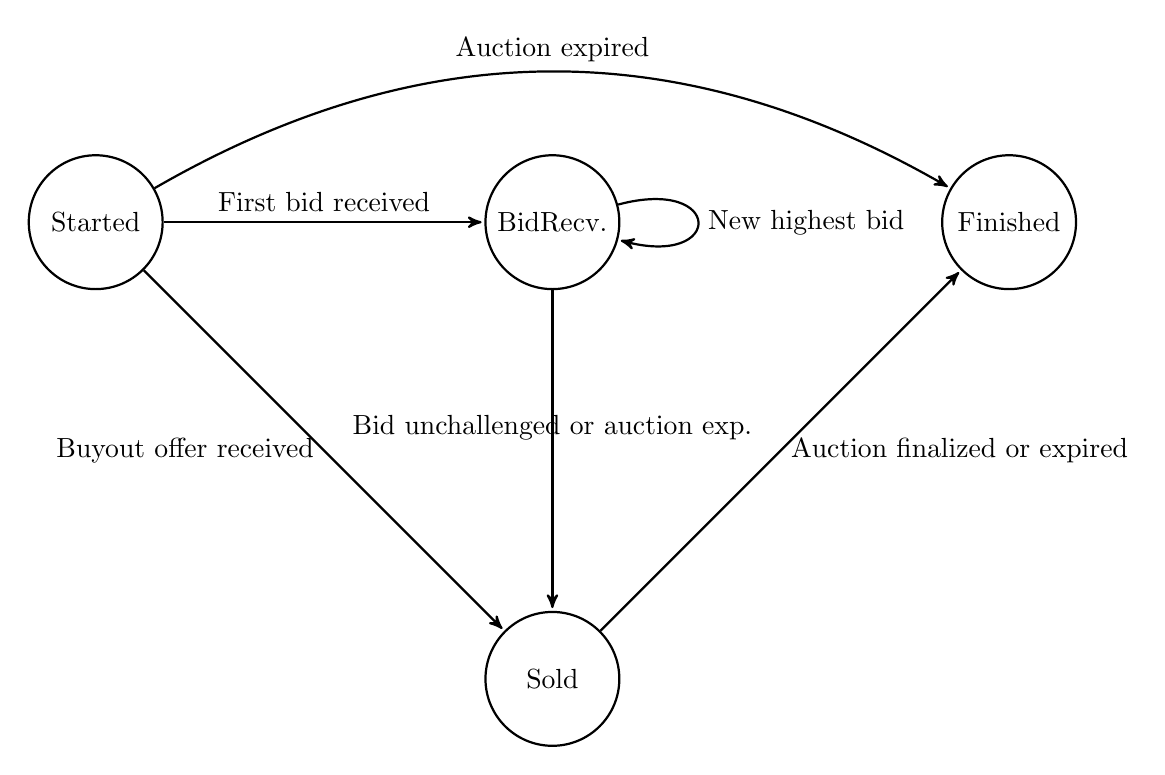
\begin{tikzpicture}[->,>=stealth',shorten >=1pt,auto,node distance=5.8cm,thick]\label{englishstates}
  \tikzstyle{every state}=[fill=white,text=black]

  \node[state, minimum size=1.7cm]         (A)                    {Started};
  \node[state, minimum size=1.7cm]         (B) [right of=A]       {BidRecv.};
  \node[state, minimum size=1.7cm]         (C) [below of=B]       {Sold};
  \node[state, minimum size=1.7cm]         (D) [right of=B]       {Finished};

  \path (A) edge [above]      node {First bid received} (B)
            edge [left]       node {Buyout offer received} (C)
            edge [bend left]  node {Auction expired} (D)
        (B) edge [loop right] node {New highest bid} (B)
        (B) edge [above]      node {Bid unchallenged or auction exp.} (C)
        (C) edge [right]      node {Auction finalized or expired} (D);
\end{tikzpicture}
\end{center}

Once again the flow of time has been implemented using the modifier \textit{blockTimedTransaction}, that is slightly different from the previous one, as shown by Listing \ref{englishtime}.

\begin{lstlisting}[language=Solidity, caption={Modifier used for modelling the time flow during an English auction, according to the automata.},captionpos=b, label=englishtime]
 modifier blockTimedTransition {
    if(phase == Phases.BidReceived && (block.number > end || block.number > bid_block+unchallenged_interval)) {
        phase = Phases.Sold; 
        emit LogSold(highest_bidder, highest_bid);
    }
    else if(phase == Phases.Started && block.number > end) {
        phase = Phases.Finished;
        emit LogPhaseTransition(phaseToString(phase));
    }
    _;
}
\end{lstlisting}

The main operations available for this kind of auction are the following:
\begin{itemize}
    \item \textit{buy\_now}: it can be invoked only in the \textit{Started} phase and its successful execution triggers a transition to the \textit{Sold} state. When invoking this function, the buyer has to provide the exact amount for the buyout, established at contract deploy time by the auctioneer or the seller. This function cannot be invoked if a bid has been already received i.e. if the contract is in the \textit{BidReceived} state, as required by the text of the assignment.
    \item \textit{bid}: this is the function for bidding. A bid is valid if it is made in the \textit{Started} phase or in \textit{BidReceived} phase (when the unchallenge period is not yet expired). The bid must be greater than the previous one plus a minimum increment specified, in percentage, at contract deploy time and stored in the variable \textit{min\_increment}. Obviously, in the case of the first bid in absolute, this function triggers a phase transition form \textit{Started} to \textit{BidReceived}.
\end{itemize}

When a bid is outbid, there is one bidder that has to be refunded: this cannot be done inside the \textit{bid} function because this would violate the \textit{Withdrawal pattern}. If a bidder wants to be refunded, he can call the \textit{withdrawal} function and get a refund.

\section{Security consideration}

Since for this project there are theoretically some money involved, guarantee the security of the systems developed is not trivial. The main risk when programming in \textit{Solidity}, excluding trivial bugs, is the re-entrancy attack: when a contract interacts with another one (e.g. transferring funds) it has to consider the possibility that the called contract can re-call it and this can result in bad behaviour such double-spending or denial of service.
In this section are described three widely used design patterns that if well implemented they guarantee an high level of protection from attacks and misbehaviour. 
\subsection{State Machine pattern}\label{statemachine}
The State Machine pattern is a behavioural pattern, useful to model systems that can be in several state with well defined rules for the transitions between states.
Contracts that fit in this scheme are often characterised by the fact that they exposed certain functionality only when they are in precise states.

This pattern when well implemented ensure that the contract exposed only the correct functionality and guarantee consistency between the different states.

Auctions are a typical scenario where this pattern is used since they are often divided into stages and at each stage the bidders are allowed to execute only certain functions. Stages in auctions are controlled by time: in this case the State Machine pattern ensures soundness in the time flow.

Implementation details for this pattern are not standard although it is very common the use of enum and struct for modelling the state and of modifiers in order to determine function exposure. The details for the code developed for this project have been described in Section \ref{english} and Section \ref{vickrey}.
\subsection{Withdrawal pattern}\label{withdrawal}
The Withdrawal pattern is a security pattern commonly used to send funds after an effect. Although it can be counterintuitive, this pattern is very powerful when the aim is to prevent a failure during a refund.

In order to understand its power let consider the following scenario. 
During an English auction, a dishonest bidder want to spend the least possible amount of ether to buy the selling good. To reach its goal the bidder make the first offer from an address associated with a contract. Next, another bidder make its bid, higher than the one of the briber. Without using the withdrawal pattern the code executed will be something similar to Listing \ref{badeng}.

\begin{lstlisting}[language=Solidity, caption={Buggy code that do not use the withdrawal pattern},captionpos=b, label=badeng]
 function bid(...) ... {
    ...
    if(msg.value > highest_bid) {
        /* refund the previous bidder*/
        highest_bidder.transfer(highest_bid);
        /*update info about winning bid*/
        highest_bidder = msg.sender;
        highest_bid = msg.value;
    }
    ...   
}
\end{lstlisting}

The problem is in line 5: \textit{highest\_bidder} contains the address of a contract owned by the briber and if this contracts has a fallback function (called by \textit{transfer}) that always fails, it will be not possible to record an offer that outbid the one of the briber and the contract it's trapped in its state. When the auction ends, the briber win the good spending the minimum amount of ether.

To implement the withdrawal pattern it is sufficient to remember who has to be refunded, for example using a mapping. When a bidder wants to withdraw his funds, he can call a specific function that make the transfer. Since the function is called by the owner of the funds, an eventual failure will only prevent the owner to recover its funds. A correct example is shown in Listing \ref{goodeng}, that differs from the previous only for line 5.

\begin{lstlisting}[language=Solidity, caption={Correct code that do use the withdrawal pattern},captionpos=b, label=goodeng]
 function bid(...) ... {
    ...
    if(msg.value > highest_bid) {
        /* refund the previous bidder*/
        pending_refunds[highest_bidder] += highest_bid;
        /*update info about winning bid*/
        highest_bidder = msg.sender;
        highest_bid = msg.value;
    }
    ...   
}
\end{lstlisting}

In the code developed, this pattern has been implemented for the English auction as shown by the above example and for the Vickrey auction for when the opening of an envelope outbid a previous winning bid.  

\subsection{Checks-Effects-Interactions pattern}\label{CEIpattern}
This security pattern has to be used when it cannot be avoided to hand over control flow to an external entity and it is desired protection against re-entrancy attacks. The C-E-I pattern is implemented in three steps:
\begin{enumerate}
    \item check the eligibility of the function invocation.
    \item adopt an optimistic accounting policy by updating the state of the contract prior a possible interaction with an external contract.
    \item interact with the external contract.
\end{enumerate}
Is possible to find a perfect example of the check-effect-interaction pattern considering the withdrawal pattern described in Section \ref{withdrawal}.

Once implemented the withdrawal pattern we have the be sure that a bidder can ask its refund exactly once. The intuitive solution is to implement a \textit{refund} function like the one in Listing \ref{badrefund}.

\begin{lstlisting}[language=Solidity, caption={Buggy refund function, vulnerable to re-entrancy attacks},captionpos=b, label=badrefund]
 function refund() public {
    require(pending_refunds[msg.sender] > 0)
    
    msg.sender.transfer(pending_refunds[msg.sender]);
    
    pending_refunds[msg.sender] = 0;
}
\end{lstlisting}

Now, the function \textit{refund} respect the check-first property but the effects, i.e. zeroing the balance of \textit{msg.sender}, are done after the interaction with an external contract. In such a situation if the \textit{transfer} in line 5 triggers a re-entrancy attack (through the fallback function) to the \textit{refund} function, \textit{msg.sender} will receive a double refund since its balance has not been updated yet.

The correct implementation is simple and requires just to swap line 4 with line 6. As a rule of thumb, when implementing this pattern, interactions (e.g. transfer, send, call etc.) should be the last commands of a function. Obviously in some cases a fail-safe policy should be implemented: if instead of \textit{transfer} I had used \textit{send}, on failure I had to update again the balance of \textit{msg.sender}.

For sake of completeness in Listing \ref{goodrefund} is shown the correct code.

\begin{lstlisting}[language=Solidity, caption={Correct refund function. Since on failure \textit{transfer} revert the transaction there is no need to check its returned value.},captionpos=b, label=goodrefund]
 function refund() public {
    require(pending_refund[msg.sender] > 0)
    
    uint refund = pending_refunds[msg.sender];
    pending_refunds[msg.sender] = 0;
    
    msg.sender.transfer(refund);
}
\end{lstlisting}

This pattern, along with the withdrawal pattern, could have mitigated the famous DAO attack that cost 3.6 million of ether.
\section{Gas consumption consideration}
\section{Testing guidelines}
\subsection{Testing Vickrey auction}
\subsection{Testing English auction}
\end{document}
